\chapter{Introducción}
\label{cap:capitulo1}
\setcounter{page}{1}

\begin{flushright}
\begin{minipage}[]{10cm}
\emph{La automatización no es el enemigo del trabajador, sino la clave para su evolución}\\
\end{minipage}\\
\end{flushright}

\vspace{1cm}

La automatización ha sido un pilar fundamental en el desarrollo de la industria moderna, permitiendo mejoras significativas en eficiencia, calidad y seguridad. Desde la evolución Industrial hasta la actualidad, la evolución de las tecnologías ha dado paso a sistemas cada vez más sofisticados, donde la integración de robots ha transformado los entornos de producción, ofreciendo resultados de mayor calidad y reduciendo costes y tiempos de producción. En particular, la robótica industrial ha desempeñado un papel clave en sectores como la automoción, la electrónica y la manufactura, ofreciendo soluciones flexibles y altamente eficientes para la producción en serie.\\

En este capítulo se presentará el contexto en el que se desarrolla este trabajo, proporcionando una visión general de la automatización en la industria y su evolución hasta la actualidad. Posteriormente, se acotará el enfoque hacia la robótica industrial, destacando su impacto en la optimización de procesos productivos. Finalmente, se delimitará el ámbito específico de este estudio, centrado en la automatización de una línea de producción robotizada, analizando sus beneficios, retos y las tecnologías empleadas.

\section{La automatización industrial}
\label{sec:miseccion} % etiqueta para luego referenciar esta sección

\subsection{Conceptos básicos de la automatización industrial}

La automatización industrial consiste en la implementación de sistemas de control, como computadoras, controladores lógicos programables (PLCs), robots y tecnologías de la información, para gestionar maquinaria y procesos productivos en el sector industrial. Su propósito principal es reducir la intervención humana, reemplazando tareas manuales, especialmente aquellas que implican riesgos, por procesos automatizados.

Este concepto surge como una evolución de la mecanización industrial, incorporando dispositivos con gran capacidad de control para optimizar la eficiencia en la fabricación. Con los avances tecnológicos y la llegada de la Industria 4.0, las empresas están modernizando sus sistemas de producción mediante el uso de control informatizado, lo que les permite mejorar la precisión, calidad y rendimiento de sus operaciones. \\

El término ``automatización'' tiene su origen en las palabras griegas ``auto'' (por sí mismo) y ``matos'' (movimiento), y se aplica a mecanismos capaces de funcionar de manera autónoma. Los sistemas automatizados ofrecen un rendimiento superior a los manuales en términos de precisión, potencia y velocidad. En el ámbito del control industrial, es posible monitorizar y regular simultáneamente diversas variables de proceso, como temperatura, flujo, presión, distancia y niveles de líquido, mediante el uso de microprocesadores o controladores de procesamiento de datos. \\

La estructura de un sistema de automatización industrial se puede representar mediante un triángulo jerárquico de tres niveles:

\begin{enumerate}
    \item \textbf{Nivel Supervisor}: Compuesto por un ordenador industrial que utiliza software especializado para el control de procesos. Su principal objetivo es la parametrización y visualización del proceso y suele utilizars el protocolo de de comunicación Ethernet industrial.
    \item \textbf{Nivel de Control}: Incluye dispositivos como PLCs que ejecutan las órdenes del nivel supervisor y controlan directamente la maquinaria en tiempo real. Estos pueden estar conectados a varios dispositivos de E/S y se comunican mediante protocolos industriales.
    \item \textbf{Nivel de Campo}: Constituido por sensores y actuadores que interactúan directamente con el proceso físico, proporcionando datos y ejecutando acciones según las instrucciones recibidas a través del bus de campo con conexión punto a punto. 
\end{enumerate}

Esta estructura permite una gestión eficiente y organizada de los procesos industriales, asegurando que cada componente funcione de manera integrada para optimizar la producción  \footnote{(N.d.). Cursosaula21.com. Retrieved March 21, 2025, from \url{https://www.cursosaula21.com/que-es-la-automatizacion-industrial/}}. 

\begin{figure} [h!]
  \begin{center}
    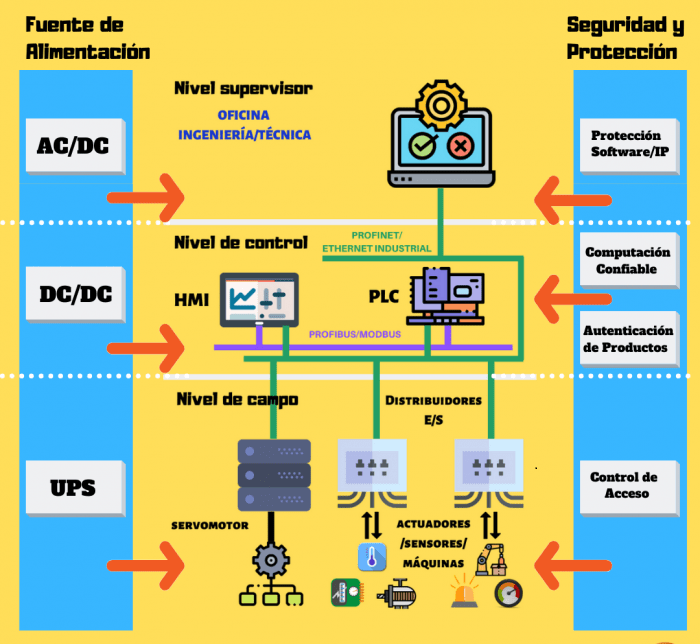
\includegraphics[width=16cm]{figs/esquema_automatizacion}
  \end{center}
  \caption{\centering Esquema de un sistema de automatización básico.}
  \label{fig:esquema_automatizacion}
\end{figure} 

\subsection{Tipos de automatización industrial}

Los sistemas de automatización industrial se clasifican principalmente en cuatro tipos según su nivel de flexibilidad y aplicación en los procesos productivos:

\begin{enumerate}
    \item \textbf{Automatización fija}: Utilizada en procesos específicos y repetitivos donde no se requieren modificaciones en el diseño del producto debido a que aplicar modificaciones resulta casi imposible. Es ideal para la producción a gran escala de productos estables.
    \item \textbf{Automatización programable}: Aplicada en la fabricación por lotes, permite modificar el proceso mediante reprogramación, aunque esto puede consumir tiempo.
    \item \textbf{Automatización flexible}: Variante más avanzada de la automatización programable, que facilita cambios rápidos y automáticos en la producción sin interrupciones significativas.
    \item \textbf{Sistema Integrado de Automatización}: Conjunto de máquinas, procesos y datos sincronizados bajo un único sistema de control. Integra herramientas como CAD, CAM, robots y sistemas de transporte automatizados para optimizar la producción.
\end{enumerate}

\subsection{Ventajas de la Automatización Industrial}

\begin{itemize}
    \item \textbf{Mayor productividad laboral}: La automatización acelera los procesos de producción, permitiendo fabricar más productos con una mejor calidad. Las nuevas tecnologías pueden operar de manera continua sin perder precisión, lo que incrementa la eficiencia y el rendimiento por hora de trabajo.
    
    \item \textbf{Mejora en la calidad del producto}: Uno de los principales beneficios de la automatización es la reducción de la cantidad de unidades defectuosas. Los sistemas automatizados garantizan una mayor uniformidad y precisión en la fabricación, cumpliendo con los estándares de calidad. Además, los procesos son supervisados en todas sus fases para asegurar un producto final óptimo.
    
    \item \textbf{Reducción de costos de producción}: La automatización permite disminuir el gasto en mano de obra al reemplazar tareas repetitivas con maquinaria, lo que reduce el costo unitario de producción. Los sistemas automatizados operan de manera constante, aumentando la eficiencia y proporcionando un alto retorno de inversión al minimizar costos laborales, ausencias y otros gastos operativos.
    
    \item \textbf{Menos trabajo manual repetitivo}: En muchas industrias, es necesario supervisar constantemente variables como temperatura, presión o nivel de líquidos. Un sistema automatizado permite gestionar estas tareas mediante controladores de lazo cerrado, reduciendo la necesidad de intervención humana en actividades rutinarias.
    
    \item \textbf{Mayor seguridad}: Al implementar un sistema automatizado, los trabajadores pasan de realizar tareas directamente en el proceso a supervisarlas, lo que disminuye los riesgos laborales. Las máquinas pueden operar en entornos peligrosos o extremos, sustituyendo a los empleados en situaciones de alto riesgo, como condiciones químicas o temperaturas elevadas, reduciendo así los accidentes laborales.
    
    \item \textbf{Facilita la monitorización remota}: Muchas operaciones industriales requieren ser controladas a distancia para una supervisión más eficiente. Los sistemas automatizados permiten la comunicación entre el área de producción y el centro de control, permitiendo a los operadores gestionar los procesos de manera remota. Un ejemplo claro de esto es el control automatizado de redes eléctricas.
\end{itemize}

\subsection{Desventajas de la Automatización Industrial}

\begin{itemize}
    \item \textbf{Aumento de la contaminación}: Muchas máquinas requieren motores que funcionan con combustibles o productos químicos que pueden generar emisiones contaminantes.
    
    \item \textbf{Menor flexibilidad}: Una máquina automatizada está diseñada para realizar tareas específicas, lo que limita la capacidad de adaptación a nuevas funciones en comparación con un trabajador humano. Actualmente, ciertas tareas, como el ensamblaje de productos con formas irregulares, siguen dependiendo del trabajo manual, aunque los avances en inteligencia artificial están cambiando esta realidad.
    
    \item \textbf{Altos costos de implementación}: La inversión inicial para adoptar un sistema automatizado es elevada. Además de los gastos en investigación y desarrollo, es necesario considerar los costos de mantenimiento, formación del personal y servicio técnico, lo que suma un desafío económico para las empresas que buscan automatizar sus procesos.
\end{itemize}

\begin{figure} [h!]
  \begin{center}
    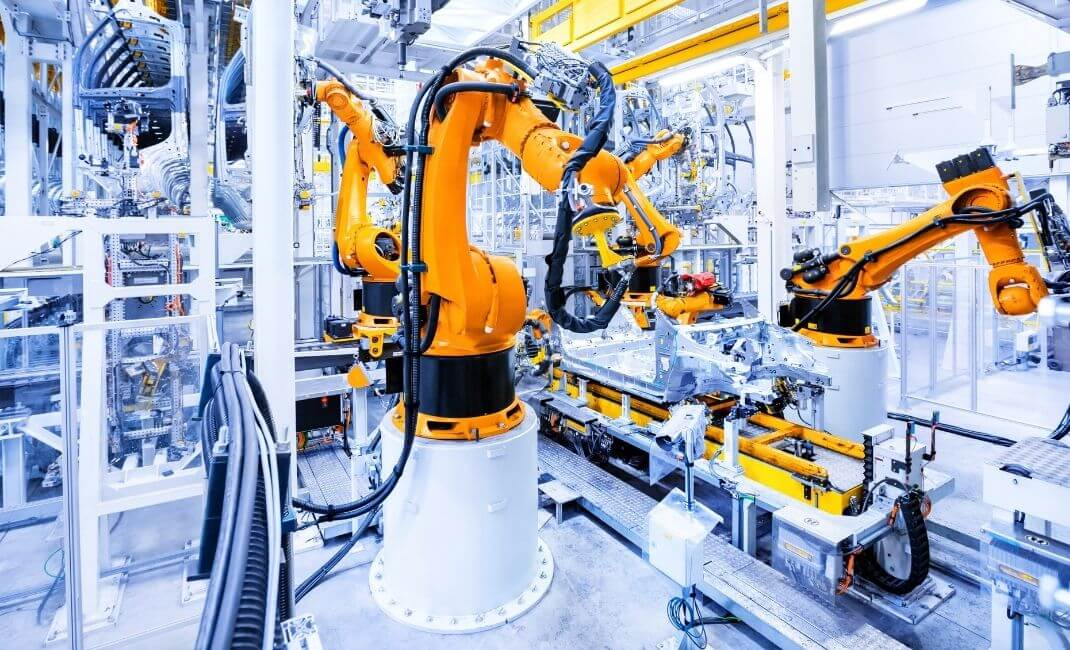
\includegraphics[width=12cm]{figs/automatizacion_industrial.jpg}
  \end{center}
  \caption{\centering Ejemplo de aplicación de automatización industrial.}
  \label{fig:automatizacion_industrial}
\end{figure}

\section{La robótica}
\label{sec:miseccion} % etiqueta para luego referenciar esta sección

La robótica es la disciplina científica que integra conocimientos de electrónica, mecánica e informática para desarrollar sistemas automatizados capaces de realizar tareas de manera autónoma o semiautónoma. Los componentes que conforman un robot son esenciales para su funcionamiento, desde la estructura mecánica (brazos, ruedas, actuadores, etc.), que debe garantizar un movimiento preciso y estabilidad, hasta los sistemas electrónicos que deben ser totalmente compatibles y funcionales para permitir la correcta operación. Además, los algoritmos que se implementan deben ser robustos, seguros y capaces de adaptarse a diversas situaciones y condiciones del entorno. \\

En el ámbito de la robótica, los sensores juegan un papel crucial, ya que proporcionan al robot la información necesaria sobre su entorno. Estos sensores, de diversos tipos, miden una amplia gama de magnitudes físicas, como la luz, posición, velocidad, fuerza, temperatura..., funcionando de manera análoga a los órganos sensoriales en los seres humanos. 

Una vez que los sensores recogen los datos del entorno, el software del robot procesa esta información, proporcionando la inteligencia necesaria para tomar decisiones. Utilizando algoritmos avanzados o inteligencia artificial, el robot es capaz de generar respuestas adecuadas a las entradas, lo que resulta en la ejecución de una acción específica, como un movimiento o la interacción con su entorno. 

Finalmente, los actuadores son los encargados de ejecutar las acciones determinadas por el sistema de control, permitiendo que el robot lleve a cabo tareas como moverse o manipular objetos. Los actuadores son fundamentales para la efectividad del robot, ya que son los elementos que materializan las decisiones procesadas en acciones físicas tangibles. 

\begin{figure} [h!]
  \begin{center}
    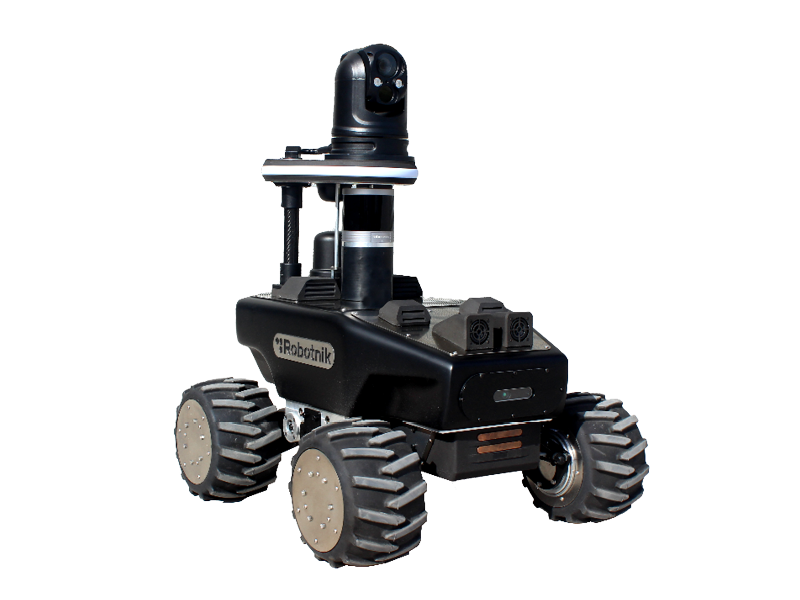
\includegraphics[width=7cm]{figs/Robot_intro}
  \end{center}
  \caption{\centering RB-WATCHER de Robotink.}
  \label{fig:Robot_intro}
\end{figure}

\subsection{Robótica Industrial}

La robótica industrial es una disciplina de la ingeniería robótica dedicada al diseño, desarrollo y fabricación de robots industriales con el propósito de automatizar tareas repetitivas tradicionalmente realizadas por seres humanos. Estos sistemas robóticos se caracterizan por seguir una secuencia de instrucciones predefinidas, ejecutando ciclos de trabajo continuos en líneas de producción de diversos sectores industriales. Su uso es particularmente frecuente en la industria manufacturera, donde contribuyen significativamente a mejorar la eficiencia, la velocidad y la calidad de los procesos productivos \footnote{(N.d.). Unir.net. Retrieved February 24, 2025, from \url{https://www.unir.net/revista/ingenieria/robotica-industrial/}}. 

A diferencia de los robots de servicio, los robots industriales operan en entornos altamente controlados, lo que simplifica su programación y control. Debido a estas condiciones estables, estos robots suelen tener más de tres grados de libertad, permitiéndoles realizar movimientos complejos con gran precisión. Aunque su aplicación principal ha sido históricamente en entornos industriales, su uso se ha expandido hacia sectores como la minería, la agricultura, el comercio y la salud, demostrando su versatilidad y adaptabilidad. 

Desde la aparición de los primeros prototipos de robots industriales, ha surgido un debate sobre su impacto en el empleo humano, con preocupaciones respecto a una posible sustitución de la mano de obra. Sin embargo, numerosos estudios sostienen que, lejos de desplazar a los trabajadores, estos sistemas robóticos buscan mejorar las condiciones laborales, eliminando tareas monótonas o peligrosas \footnote{Robótica industrial: Qué es, usos y aplicaciones. (2023, June 14). Computing. \url{https://www.computing.es/informes/robotica-industrial-que-es-usos-aplicaciones/}}. 

\begin{figure} [h!]
  \begin{center}
    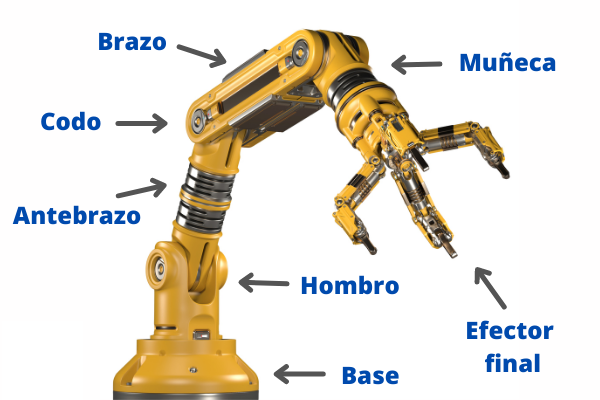
\includegraphics[width=9cm]{figs/brazo_industrial}
  \end{center}
  \caption{\centering Partes de un brazo robótico industrial.}
  \label{fig:brazo_industrials}
\end{figure}

\section{Evolución e historia de la robótica industrial}
\label{sec:segundaseccion}

La robótica industrial aparece por primera vez a mediados del siglo XX en Europa a manos del británico Bill Taylor, estudiante que sobre 1937 creó el robot Gargantua, un robot en forma de grua cuya principal función era la colocación de objetos, dando lugar al primer modelo de pick \& place \footnote{Marketing. (2021, February 2). Historia y Evolución de la Robótica Industrial. EDS Robotics. \url{https://www.edsrobotics.com/blog/evolucion-robotica-industrial/}}. 

Por otro lado, George Devol fue el encargado de crear la primera empresa de robótica de la historia llamada \textit{Unimation} y en el año 1954 se crea el que se considera el primer robot industrial. Este robot consistía en un brazo hidráulico cuya finalidad era elevar cargas pesadas para facilitar su transporte, y en los años siguientes se fueron sacando versiones más avanzadas de este modelo. Además, esta empresa participó en el desarrollo del primer robot de transferencia programable en 1961 \footnote{Robotnik, P. (2021, November 2). Historia \& Origen de los Robots y de la Robótica. Robotnik. \url{https://robotnik.eu/es/historia-de-los-robots-y-la-robotica/}}. \\


\begin{figure}[ht!]
	\centering
	\begin{minipage}{0.44\linewidth}
		\centering
		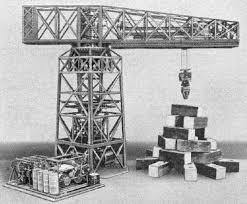
\includegraphics[width=\linewidth]{figs/gargantua.jpg}
		\caption*{\centering Gargantua.}
	\end{minipage}
	\begin{minipage}{0.52\linewidth}
		\centering
		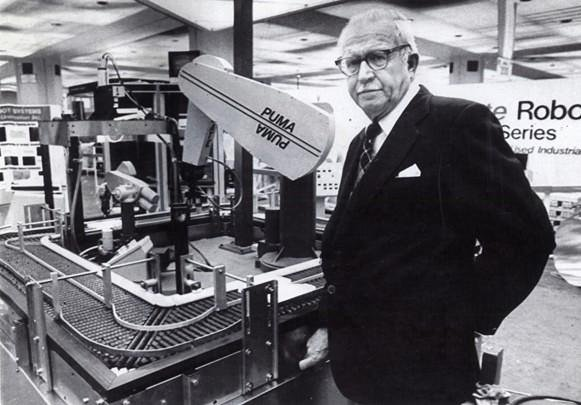
\includegraphics[width=\linewidth]{figs/George_Devol}
		\caption*{\centering George Devol.} 
	\end{minipage}
	\caption{Primeros robots industriales.}
	\label{fig:ancientrel}
\end{figure}

En los años 60 y 70 ya empezaron a aparecer modelos de brazos robóticos más elaborados y de mayor tamaño con elementos como sensores o cámaras incorporados en ellos. En 1973 la empresa alemana KUKA crea Famulus, el primer robot industrial con motores eléctricos y en 1974 Victor Scheinman desarrolla el robot PUMA (Programmable Universal Machine for Assembly), el cual se convierá en un estándar en la industria \footnote{Sutori. (n.d.). Sutori.com. Retrieved February 24, 2025, from \url{ https://www.sutori.com/es/historia/linea-de-tiempo-evolucion-de-la-robotica-industrial--6w6pytow1tj3grr5scVKU1Ns}}. \\

En los años 80 la robótica industrial alcanzó su máximo desarrollo debido a que la fabricación y venta de esta aumentó un 80\% y, aunque EEUU fue el impulsor de esta industria, también empezó a desarrollarse en Asia y Europa. Destaca el robot Motoman L10 de Yaskawa desarrollado en 1981, el cual introduce el uso de retroalimentación por visión, lo que permite a los robots la identificación de objetos y su entorno o el PUMA 560, primer prototipo de robot quirúrgico. 

A partir de la década de 1990, la robótica industrial experimentó un crecimiento significativo, impulsado por la globalización y la creciente demanda de bienes de consumo. Este período marcó la transición hacia la robótica inteligente, estableciendo estándares internacionales por la (ISO) y utilizando sensores avanzados dando lugar a mejores resultados. 

\begin{figure}[ht!]
	\centering
	\begin{minipage}{0.39\linewidth}
		\centering
		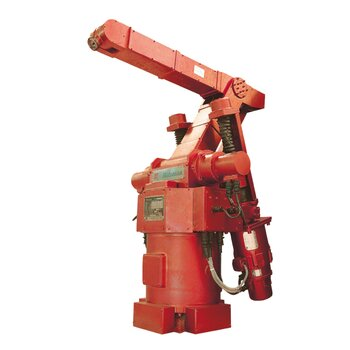
\includegraphics[width=\linewidth]{figs/motoman.jpg}
		\caption*{\centering Motoman L10.}
	\end{minipage}
	\begin{minipage}{0.59\linewidth}
		\centering
		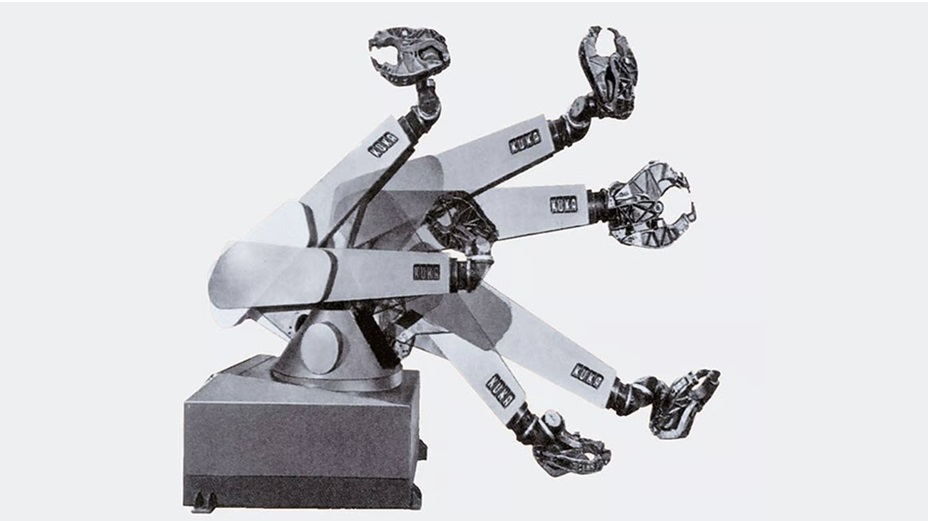
\includegraphics[width=\linewidth]{figs/famulus.jpg}
		\caption*{\centering Famulus.} 
	\end{minipage}
	\caption{Robots industriales pupulares en la década de los 70.}
	\label{fig:ancientrel}
\end{figure}

Entrando al siglo XXI se crean los primeros robots colaborativos, conocidos como cobots, concebidos para cooperar de manera directa con las personas. Estos dispositivos se caracterizan por su seguridad, adaptabilidad y facilidad de programación, convirtiéndose en una solución ideal para entornos industriales donde es necesario combinar tareas manuales y automatizadas. 

En los años 2010, la Industria 4.0 emergió como una nueva fase en la manufactura, caracterizada por la digitalización y la interconexión de sistemas de producción.  Los robots industriales se convirtieron en componentes clave de las fábricas inteligentes, colaborando estrechamente con humanos y otros sistemas automatizados para optimizar la eficiencia y la flexibilidad en la producción. 

\section{Tipos de robots industriales}
\label{sec:terceraseccion}

En este apartado se van a abordar los conceptos esenciales de la robótica industrial, proporcionando una visión general de los distintos tipos de robots, sus componentes principales y las distintas técnicas existentes para operar con ellos. Comprender estos fundamentos es crucial para desarrollar soluciones eficientes y optimizar los procesos de producción.

 Según la norma internacional ISO 8373:2012 un robot industrial se define como ``un manipulador multifuncional, reprogramable y controlado automáticamente, programable en tres o más ejes que puede estar fijo en un área o móvil para su uso en aplicaciones de automatización industrial''. Todo ello a partir de trayectorias variables para ejecutar diversas tareas cíclicas y adaptables. \footnote{Tipos de robots industriales: clasificación y características. (2020, June 2). Esneca; Esneca Business School. 
 \url{ https://www.esneca.lat/blog/tipos-robots-industriales-caracteristicas/}}. 
 
Existen una gran variedad de diseños y configuraciones de robots industriales debido a las diversas aplicaciones y entronos en los que estos se emplean. Esta clasificación puede realizarse según diversos criterios, siendo el más común el tipo de configuración mecánica, que determina los grados de libertad, el alcance y la versatilidad del robot.

\subsubsection{Robot cartesiano}

Los robots cartesianos se componen de tres articulaciones prismáticas y utilizan el sistema de coordenadas tridimensionales, el cual lo forman los ejes X, Y y Z. Los movimientos de estos robots son lineales por lo que su funcionamiento es sencillo y se limita a movimiento de traslación. Suelen ser utilizados para mover cargas pesadas linealmente en las que no es necesario rotarlas\footnote{(N.d.). Sicma21.com. Retrieved March 12, 2025, from  \url{https://www.sicma21.com/robots-industriales-tecnologia-y-aplicaciones/}}. 

\begin{figure} [h!]
  \begin{center}
    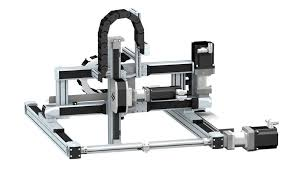
\includegraphics[width=7cm]{figs/robot_cartesiano}
  \end{center}
  \caption{\centering Robot cartesiano.}
  \label{fig:robot_cartesiano}
\end{figure} 

\subsubsection{Robot antropomórfico}

Estos robots articulados son los más comunes en el sector de fabricación enfocados en aplicaciones complejas como el montaje de productos, soldadura o mecanizado. El ``end effector'' (pieza situada en el extremo final del brazo) poseen seis grados de libertad para poder operar en cualquier situación. Los brazos de este estilo poseen tres articulaciones de giro y otra opcional en el EOAT.

\begin{figure} [h!]
  \begin{center}
    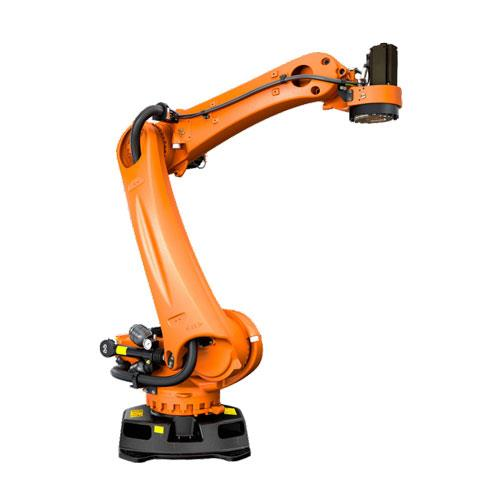
\includegraphics[width=6cm]{figs/robot_antropomorfico}
  \end{center}
  \caption{\centering Robot antropomórfico.}
  \label{fig:robot_antropomorfico}
\end{figure} 

\subsubsection{Robot cilíndrico}

Los robots cilíndricos se caratcerizan por tener movimientos cilíndricos debido a que están compuestos de dos articulaciones prismáticas y otra de revolución. Esta morfología le permite movimientos de rotación en torno a su propio eje y con las articulaciones prismáticas ajusta la altitud y radio de trabajo. Su principal aplicación es la de ``pick and place'' las cuales no requieren desplazamiento.

\begin{figure} [h!]
  \begin{center}
    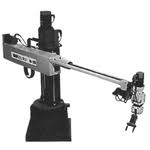
\includegraphics[width=5.5cm]{figs/robot_cilindrico}
  \end{center}
  \caption{\centering Robot cilíndrico.}
  \label{fig:robot_cilindrico}
\end{figure} 

\subsubsection{Robot SCARA}

Este tipo de robots tiene como peculiaridad que poseen un brazo con libertad en un plano XY, pero con restricción de movimiento en el eje Z. Estos modelos están formados por dos eslabones en adición a dos juntas de revolución y una prismática. La función de la articulación prismática es desplazar en el eje Z el EOAT y tiene diversas aplicaciones como la paletización, el ensambalaje o biomedicina.

\begin{figure} [h!]
  \begin{center}
    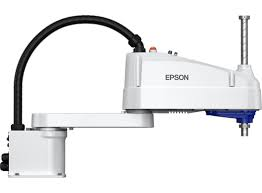
\includegraphics[width=6cm]{figs/robot_SCARA}
  \end{center}
  \caption{\centering Robot SCARA.}
  \label{fig:robot_SCARA}
\end{figure} 

\subsubsection{Robot delta}
Los robots delta están formados por tres eslabones unidos al un EOAT mediante tres juntas universales y una base común. La base está formada por tres juntas primáticas o accionadas por revoluciones y su función es proporionarle cuatro grados de libertad al EOAT para que pueda moverse en todos los ejes cartesianos y girar sobre su eje Z. Sus principales aplicaciones son la de ``pick and place'' de forma veloz en la industria alimentaria, electrónica y farmacéutica.


\begin{figure} [h!]
  \begin{center}
    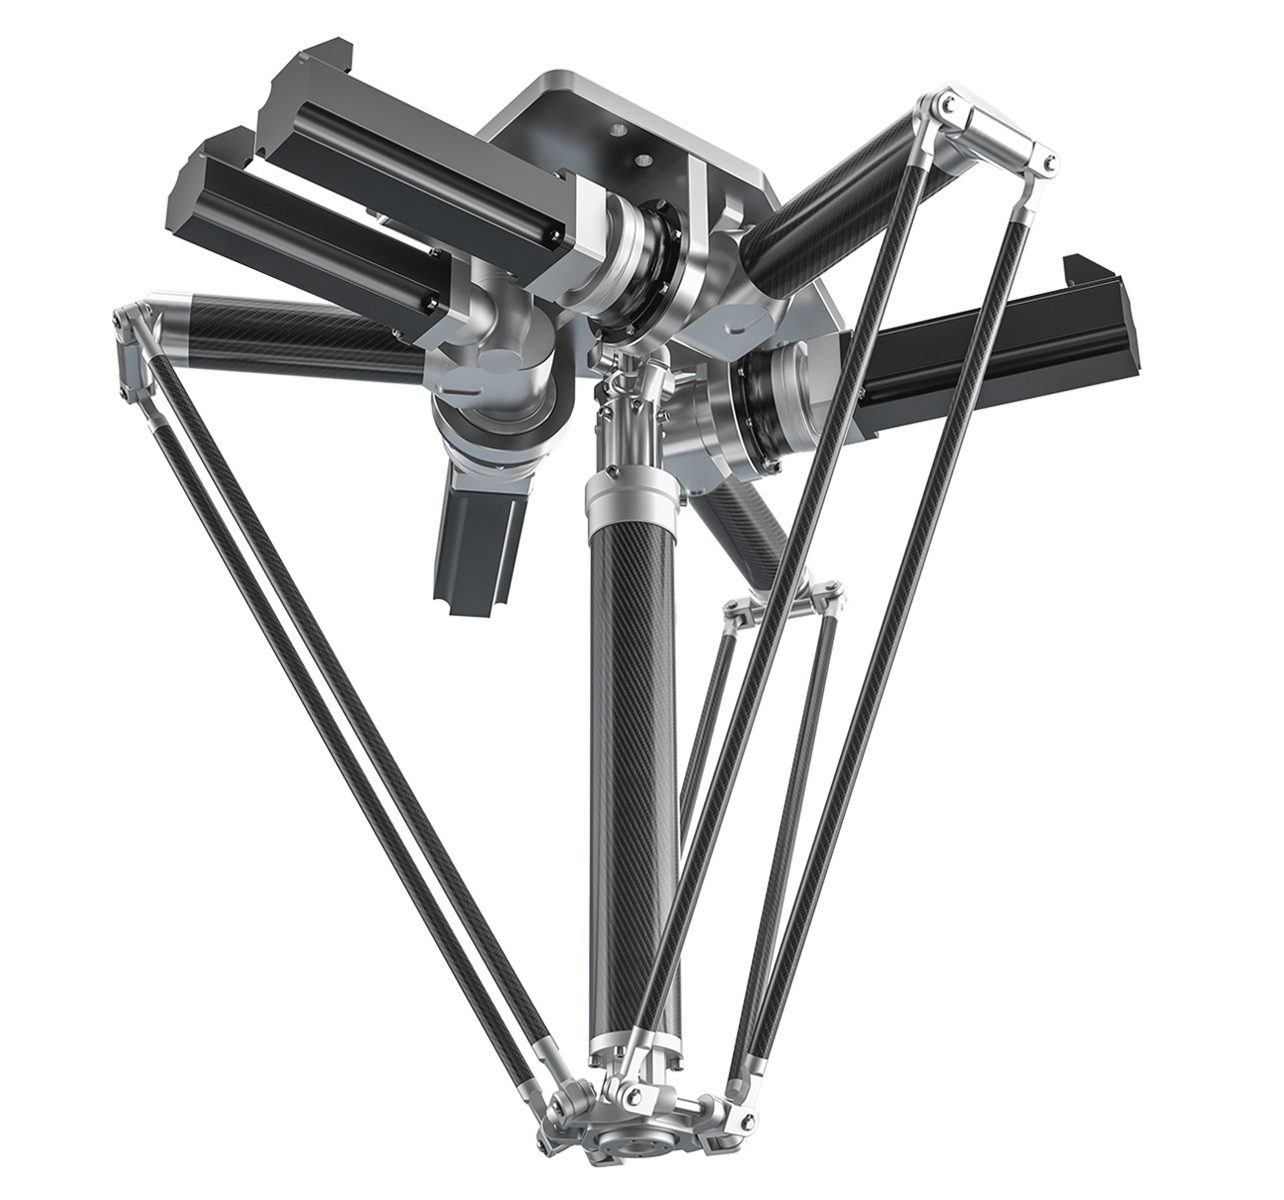
\includegraphics[width=6cm]{figs/robot_delta}
  \end{center}
  \caption{\centering Robot delta.}
  \label{fig:robot_delta}
\end{figure} 

\subsubsection{Robot esférico}

Estos robots también tienen el nombre de robots polares y están basados en el sistema de coordenadas polares consiguiendo un área de trabajo esférica. La longitud del enlace entre el EOAT y la articulación de revolución más cercana establecen su rango de movimiento permitiendo un mayor alcance en comparación a otros modelos. So aplicación más común es en aplicaciones de carga de mñaquinas debido a su largo alcance.

\begin{figure} [h!]
  \begin{center}
    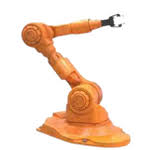
\includegraphics[width=5cm]{figs/robot_esferico}
  \end{center}
  \caption{\centering Robot esférico.}
  \label{fig:robot_esferico}
\end{figure} 


\section{Motivación del trabajo}
\label{sec:quintaseccion}

En los textos puedes poner palabras en \textit{cursiva}, para aquellas expresiones en sentido \textit{figurado}, palabras como \textit{robota}, que está fuera del diccionario castellano, o bien para resaltar palabras de una colección: \textit{(a)} es la primera letra del abecedario, \textit{(b)} es la segunda, etc.\\



No olvides incluir imágenes y referenciarlas, como la Figura \ref{fig:Robot_intro}.

\subsection{Números}
\label{sec:subseccion}

En lugar de tener secciones interminables, como la Sección \ref{sec:miseccion}, divídelas en subsecciones.

Para hablar de números, mételos en el entorno \textit{math} de \LaTeX, por ejemplo, $1.5Kg$. También puedes usar el símbolo del Euro como aquí: 1.500\euro.

\subsection{Listas}

Cuando describas una colección, usa \texttt{itemize} para ítems o \texttt{enumerate} para enumerados. Por ejemplo:

\begin{itemize}
 \item \textit{Entorno de simulación.} Hemos usado dos entornos de simulación: uno en 3D y otro en 2D.
 \item \textit{Entornos reales.} Dentro del campus, hemos realizado experimentos en Biblioteca y en el edificio de Gestión.
\end{itemize}\

\begin{enumerate}
 \item Primer elemento de la colección.
 \item Segundo elemento de la colección.
\end{enumerate}\

\paragraph{Referencias bibliográficas}
\label{sec:referencias}

Cita, sobre todo en este capítulo, referencias bibliográficas que respalden tu argumento. Para citarlas basta con poner la instrucción \verb|\cite| con el identificador de la cita. Por ejemplo: libros como \cite{vega12e}, artículos como \cite{vega19b}, URLs como \cite{vega19a}, tesis como \cite{vega18b}, congresos como \cite{vega18a}, u otros trabajos fin de grado como \cite{vega08b}.

Las referencias, con todo su contenido, están recogidas en el fichero \texttt{bibliografia.bib}. El contenido de estas referencias está en formato \texttt{BibTex}. Este formato se puede obtener en muchas ocasiones directamente, desde plataformas como \texttt{Google Scholar} u otros repositorios de recursos científicos.

Existen numerosos estilos para reflejar una referencia bibliográfica. El estilo establecido por defecto en este documento es APA, que es uno de los estilos más comunes, pero lo puedes modificar en el archivo \texttt{memoria.tex}; concretamente, cambiando el campo \verb|apalike| a otro en la instrucción \verb|\bibliographystyle{apalike}|. 

\

\

\

Y, para terminar este capítulo, resume brevemente qué vas a contar en los siguientes.
